\chapter{État de l'art}

Dans cette section, nous allons détailler tous les outils à notre disposition ainsi que leur fonctionnement.

\section{Techniques de reconnaissance d'écriture}

La plupart des techniques de reconnaissance de l'écriture sont basées sur des classifieurs
dits dynamiques, c'est-à-dire qu'ils possèdent une mémoire interne ou possèdent une notion
de contexte dans leur analyse. Ces classifieurs permettent un parcours et une division des
données d'entrées et donc d'effectuer une classification pour chacune des divisions repérées. 
		
\subsection{Modèles de Markov Cachés}

Les Modèles de Markov Cachés (MMC) sont des modèles probabilistes basés sur une structure de
graphe d'états. Ils modélisent une séquence basée sur des connaissances \textit{a priori},
comme un langage pourrait être défini à l'aide de la forme des lettres. Les probabilités de passage
d'un état à un autre dépendent d'une matrice de transition et un vecteur de conditions initiales
permet de définir l'état de départ. Les MMC permettent de modéliser la probabilité de choisir un caractère
en fonction de l'état actuel du système de reconnaissance. Pour cela, les différentes composantes
de l'alphabet utilisé sont décomposées (première partie de boucle du \texttt{d}, barre verticale du \texttt{l}, etc).
Ces composantes correspondent aux états du graphe. On pourra donc modéliser la
probabilité pour un système de choisir un \texttt{l} après avoir lu une barre verticale, etc.
Ces probabilités ne seront pas égales à 1 car une barre verticale peut aussi correspondre à un
\texttt{t} par exemple. Cependant, cette approche impose une segmentation des composantes
de l'alphabet que l'on souhaite traiter et impose de changer ces composantes ou d'étendre
l'alphabet reconnu. Or, cette segmentation et l'étiquetage correspondant ("c'est une boucle d'un a", etc)
ne sont pas toujours évidents et peuvent être fastidieux à faire.

\paragraph{}
\begin{mdframed}[frametitle={Schéma de transition et d'observation d'un MMC}, innerbottommargin=10]
\begin{center}
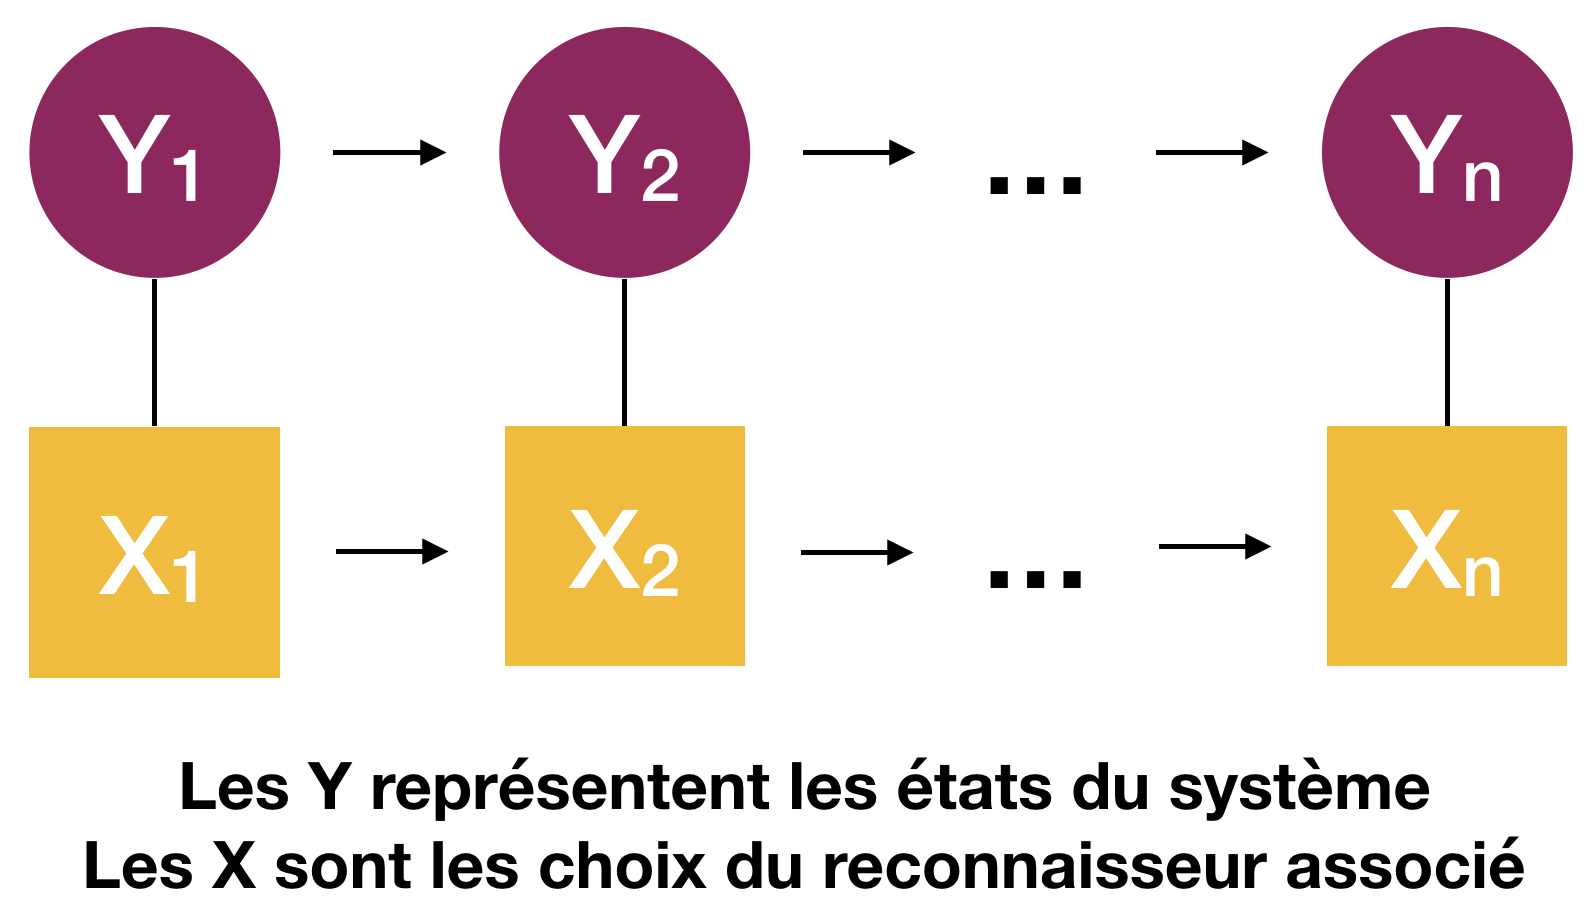
\includegraphics[width=0.6\linewidth]{mmc.png}
\end{center}
\end{mdframed}

\subsection{Champs Aléatoires Conditionnels}

Les Champs Aléatoires Conditionnels sont des modèles basés également sur des probabilités et
sur une structure similaire aux MMC. La principale différence entre ces deux méthodes est que pour les MMC,
les probabilités de choix des caractères dépendent d'un état, tandis que pour les CAC, le choix d'un
caractère peut être réalisé depuis n'importe quel état, avec une pondération par un potentiel.
Cette approche permet alors de prendre en compte l'ensemble du contexte local de la séquence observée
du fait de l'hypothèse de non-indépendance des états. Ce modèle est donc plus approprié pour l'analyse de
séquences structurées. Cependant, ils n'effectuent pas d'étiquetage de séquence lors de leur apprentissage,
et ne possèdent pas de structuration interne qui leur permettrait de saisir des structures de plus haut
niveau telles que les titres ou la date dans un document.

\paragraph{}
\begin{mdframed}[frametitle={Schéma de transition et d'observation d'un CAC}, innerbottommargin=10]
\begin{center}
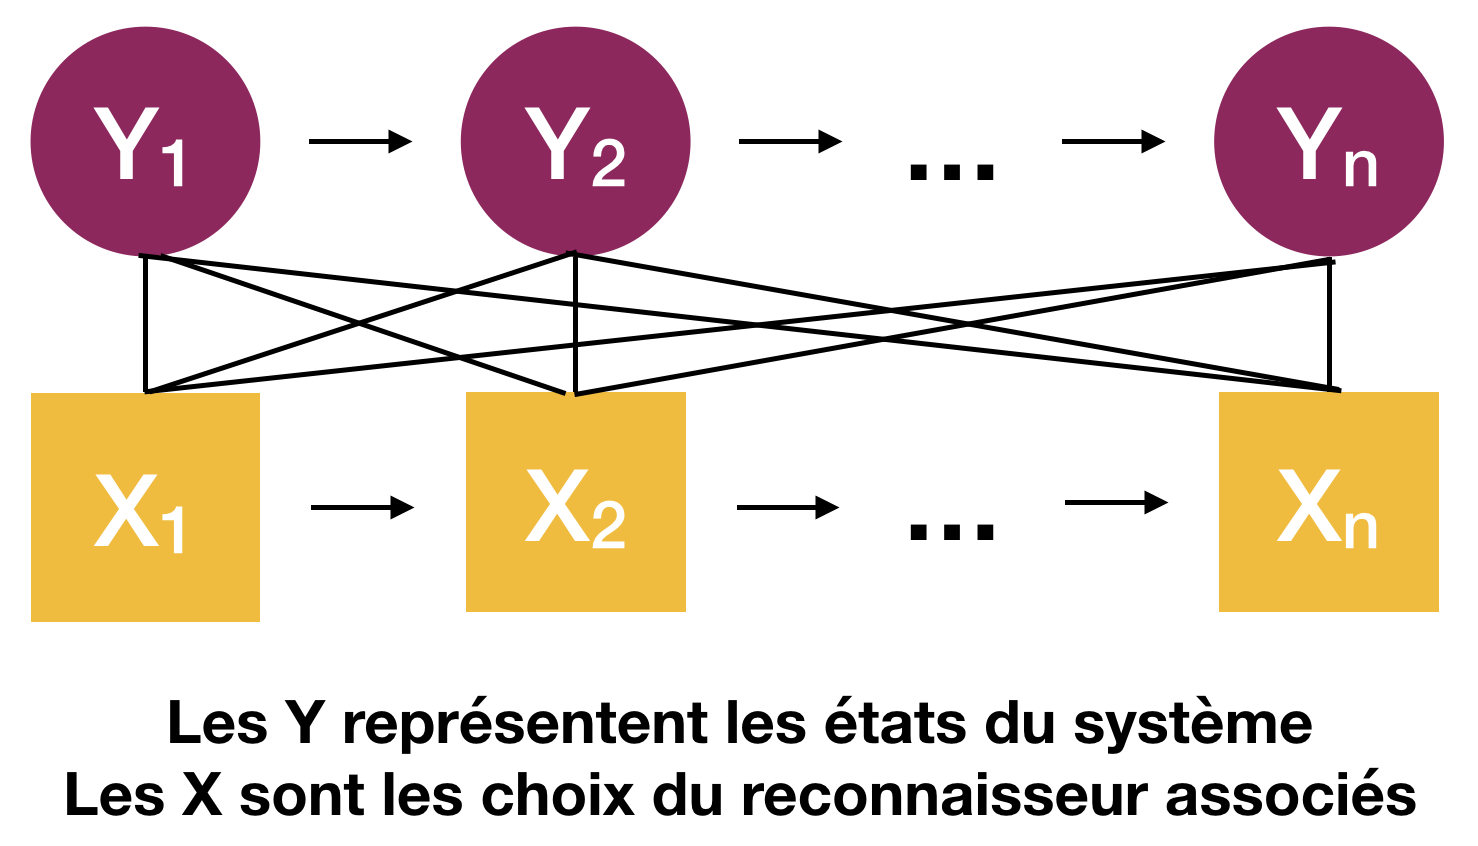
\includegraphics[width=0.6\linewidth]{cac.png}
\end{center}
\end{mdframed}

\subsection{Réseaux de Neurones Récurrents}

Les Réseaux de Neurones Récurrents sont basés sur la structure classique des réseaux de neurones,
avec une modification : chaque neurone des couches cachées possède également en entrée les sorties
des neurones correspondant à leur couche. Ceci permet d'avoir une mémoire interne des états de chaque couche.
Via cette approche, il n'est pas nécessaire d'effectuer un étiquetage des données car le réseau apprend
par lui-même. Cette méthode apporte également une vue plus globale de l'ensemble d'entrée car on ne se limite
pas à l'observation d'un état précédent. Le principal soucis de ces réseaux provient de l'apprentissage.
Ils nécessitent un grand jeu de données et on remarque une "disparition" du gradient sur les couches les plus
profondes, c'est-à-dire que les poids d'entrée ne sont que peu modifiés lors de l'apprentissage. Il faut alors
recourir à un apprentissage couche par couche, ce qui est compliqué à cause de la récurrence de ce type de réseaux.

\subsection{Réseaux de Neurones Récurrents Multi-Dimensionnels}

Les MDRNN sont conçus afin d'apporter une localité et une mémoire sur les deux dimensions de l'image traitée.
Ils sont constitués de couches de réseaux de neurones de différentes natures organisés selon l'abstraction des
données à effectuer. L'image est tout d'abord décomposée en blocs. Des réseaux récurrents la parcourent alors
en la transformant dans chaque direction diagonale. Les sorties de ces réseaux sont alors transmises à un
réseau convolutionnel qui permet d'augmenter le niveau d'abstraction des données de sortie.

\newpage

\begin{mdframed}[frametitle={Schéma de structure d'un MDRNN}, innerbottommargin=10]
\begin{center}
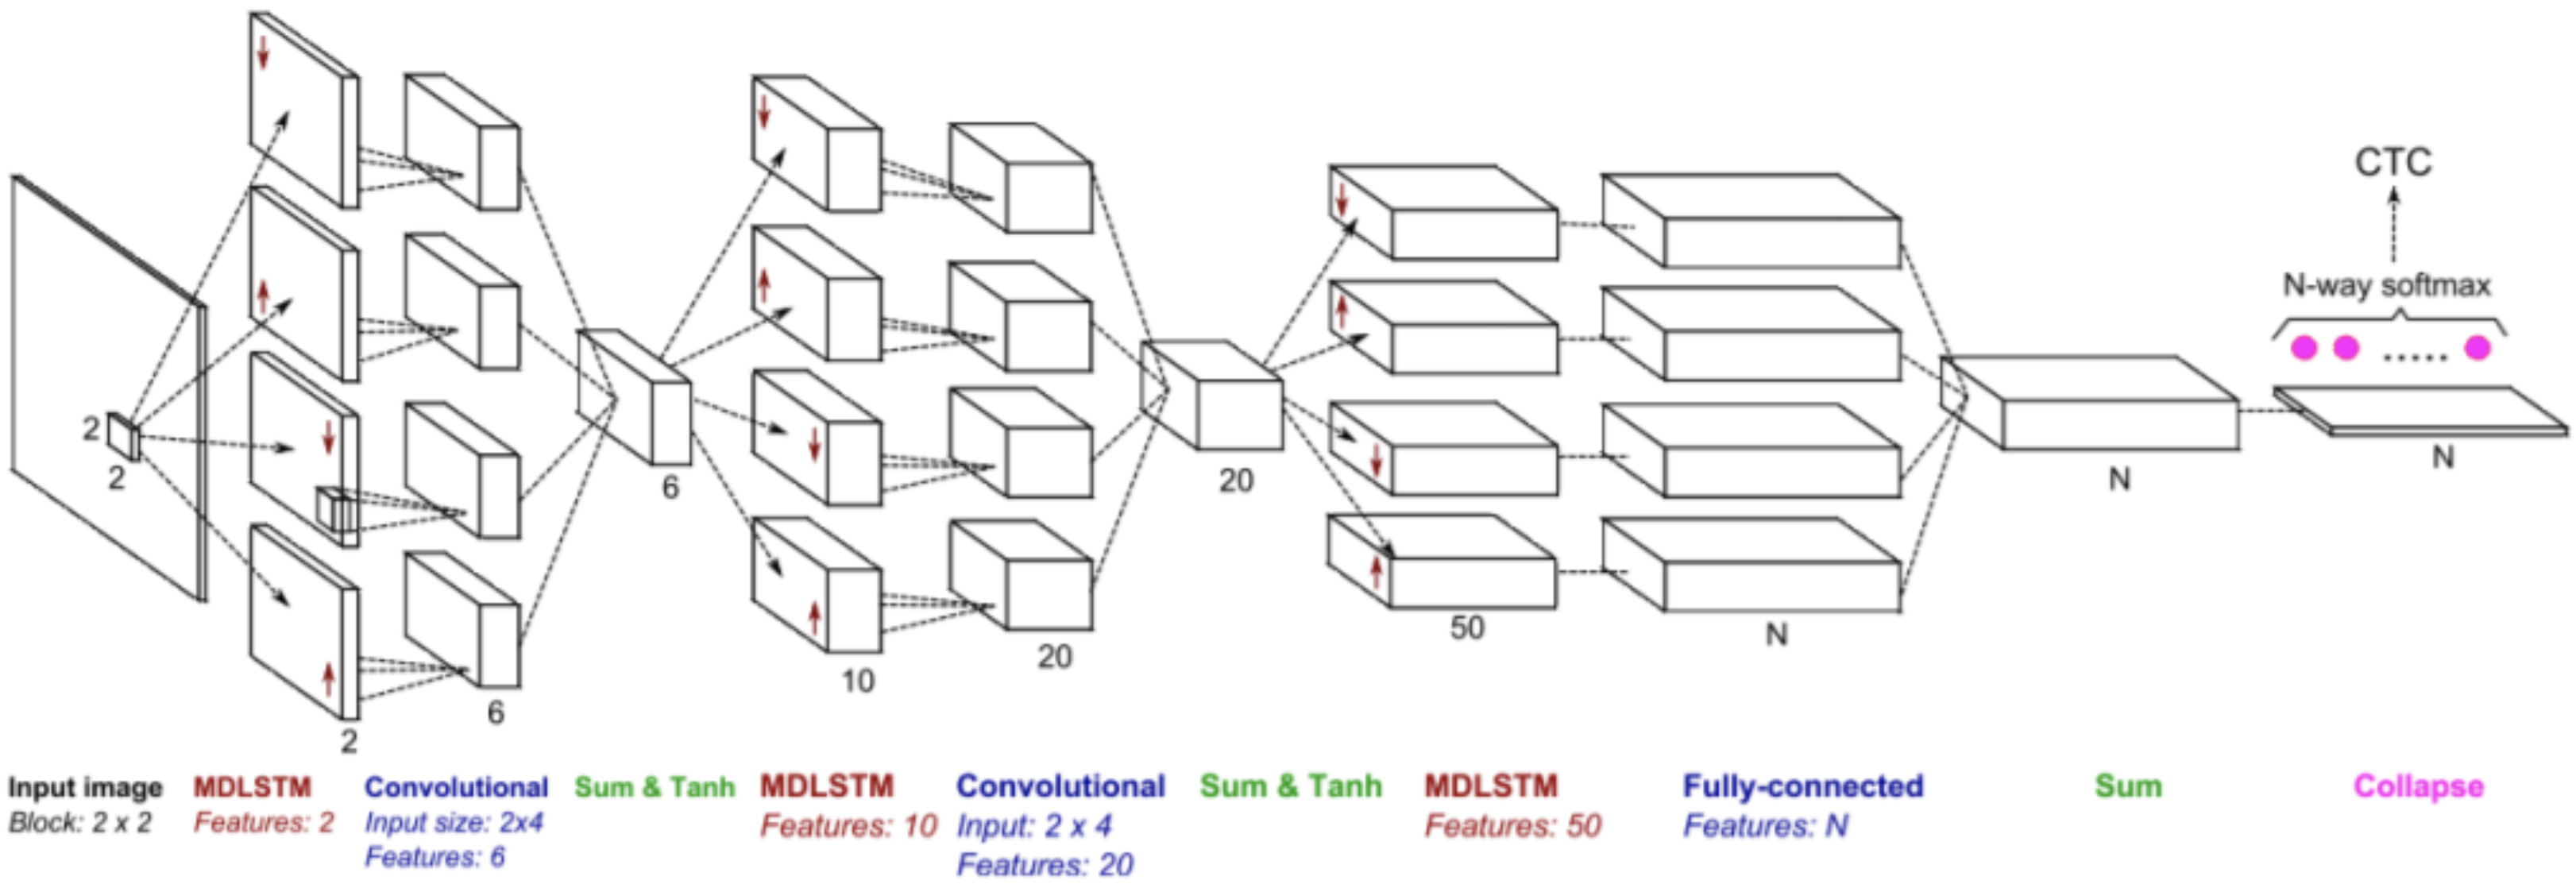
\includegraphics[width=0.6\linewidth]{mdrnn.png}
\end{center}
\end{mdframed}

\paragraph{}
Cependant, cette structure ne permet pas une segmentation de l'image de départ. Il est donc nécessaire de créer
cette segmentation afin d'établir une relation entre les données d'entrée et les sorties. Afin de réaliser cette
segmentation, une adaptation des algorithmes d'apprentissage est nécessaire.

\section{Détecteur de lignes}

\subsection{Par floutage}

\subsection{Par réseau de neurone à convolution}

\section{Format de description d'image}

\subsection{GEDI}

GEDI est un outil qui permet d'annoter des documents scannés. Il est ainsi très utile pour établir
la vérité terrain. Il met en scène deux types de documents : des images qui correspondent aux documents
scannés ainsi que des documents XML au format GEDI qui permettent de stocker toutes les informations
relatives aux documents scannés. On peut alors avoir, pour chaque document scanné, des informations
relatives à la position des paragraphes, à la langue dans laquelle le texte est écrit, ou encore à
la forme du texte (manuscrit ou imprimé). La vérité terrain que nous aurons au sein de notre projet
aura été établie avec GEDI.

\subsection{PiFF}

Le Pivot File Format (PiFF) est un format de description d'image basé sur JSON et créé par différents
chercheurs français, dont notre encadrant de projet, Bertrand COÜASNON. Ce format est très utile pour l'analyse
de documents puisqu'il permet le partage de jeu de données, le traitement de résultats ainsi que
l'utilisation d'outils déjà existants sans avoir à faire de conversion entre les différents formats
qui pourraient exister. De ce fait, les différentes étapes de l'analyse de documents peuvent être effectuées
par différentes équipes sans qu'il n'y ait de conflit au niveau du format des données, ce qui permet une
collaboration plus facile. Les données présentes en entrée dans le cas de notre projet seront au format PiFF.
Par conséquent, les données après traitement par le logiciel devront également être dans ce format.